\documentclass[10pt,a4paper]{extarticle}

% English version — compile with XeLaTeX (Latin Modern, same Latin font as main.tex)
\usepackage{fontspec}
\usepackage[left=1.2cm, right=1.2cm, top=0.8cm, bottom=0.8cm]{geometry}
\usepackage{enumitem}
\usepackage{titlesec}
\usepackage{hyperref}
\usepackage{xcolor}
\usepackage{graphicx}
\usepackage{tikz}

% ========== Compact line spacing ==========
\linespread{1.12}

% Never hyphenate method / benchmark names (e.g. CK-MIL, Struc-tAttack)
\hyphenation{CKMIL StructAttack ReMAP MuirBench SafeBench Selector Consumer}
\emergencystretch=1em

% UESTC primary blue
\definecolor{uestcblue}{HTML}{004098}

\hypersetup{
    colorlinks=true,
    linkcolor=uestcblue,
    filecolor=uestcblue,
    urlcolor=uestcblue,
}

% ---------- Section icons (TikZ vector paths) ----------
\newcommand{\educationicon}{%
    \tikz[baseline=-0.22em,x=1.08em,y=1.08em,line width=0.07em,line cap=round,line join=round]{%
        \draw[uestcblue] (0,0.18)--(0.50,0.40)--(1,0.18)--(0.50,-0.04)--cycle;
        \draw[uestcblue] (0.20,0.10)--(0.20,-0.10) .. controls (0.38,-0.27) and (0.62,-0.27) .. (0.80,-0.10)--(0.80,0.10);
        \draw[uestcblue] (1,0.18)--(1,-0.14);
        \fill[uestcblue] (1,-0.18) circle (0.055);
    }%
}
\newcommand{\researchicon}{%
    \tikz[baseline=-0.25em,x=0.94em,y=0.94em,line width=0.07em,line cap=round,line join=round]{%
        \draw[uestcblue] (0.34,0.42)--(0.34,0.10)--(0.12,-0.28) .. controls (0.04,-0.43) and (0.18,-0.48) .. (0.50,-0.48) .. controls (0.82,-0.48) and (0.96,-0.43) .. (0.88,-0.28)--(0.66,0.10)--(0.66,0.42);
        \draw[uestcblue] (0.27,0.42)--(0.73,0.42);
        \draw[uestcblue] (0.22,-0.18) .. controls (0.36,-0.10) and (0.64,-0.26) .. (0.78,-0.18);
    }%
}
\newcommand{\skillsicon}{%
    \tikz[baseline=-0.25em,x=0.94em,y=0.94em,line width=0.08em,line cap=round,line join=round]{%
        \draw[uestcblue] (0.31,0.34)--(0.04,0)--(0.31,-0.34);
        \draw[uestcblue] (0.69,0.34)--(0.96,0)--(0.69,-0.34);
        \draw[uestcblue] (0.59,0.42)--(0.41,-0.42);
    }%
}
\newcommand{\awardicon}{%
    \tikz[baseline=-0.25em,x=0.94em,y=0.94em,line width=0.07em,line cap=round,line join=round]{%
        \draw[uestcblue] (0.22,0.38)--(0.29,-0.01) .. controls (0.32,-0.18) and (0.42,-0.24) .. (0.50,-0.24) .. controls (0.58,-0.24) and (0.68,-0.18) .. (0.71,-0.01)--(0.78,0.38)--cycle;
        \draw[uestcblue] (0.23,0.28) .. controls (0.02,0.28) and (0.02,-0.03) .. (0.30,-0.06);
        \draw[uestcblue] (0.77,0.28) .. controls (0.98,0.28) and (0.98,-0.03) .. (0.70,-0.06);
        \draw[uestcblue] (0.50,-0.24)--(0.50,-0.42);
        \draw[uestcblue] (0.31,-0.42)--(0.69,-0.42);
    }%
}

% Section style: UESTC blue title with rule
\titleformat{\section}{\large\bfseries\raggedright\color{uestcblue}}{}{0em}{}[\color{uestcblue}\titlerule]
\titlespacing{\section}{0pt}{4pt}{3pt}

\setlength{\parskip}{1pt}

% ---------- Project heading: arrow, area, dates ----------
\newcommand{\projecticon}{%
    \tikz[baseline=-0.03em,x=0.90em,y=1.30em,line join=round]{%
        \fill[black!72] (0,0.42)--(0.65,0.21)--(0,0)--(0.15,0.21)--cycle;
    }%
}
\newcommand{\projectheading}[2]{%
    \noindent\projecticon\hspace{0.28em}\textbf{#1}\hfill\textbf{#2}\par\vspace{2pt}
}
\newcommand{\projectseparator}{%
    \par\vspace{3pt}%
    {\color{uestcblue!28}\hrule height 0.35pt}%
    \vspace{2pt}%
}

% ---------- Research entry: heading line, then paper title ----------
\newcommand{\researchentry}[3]{%
    \projectheading{#1}{#2}
    \noindent{\color{uestcblue}\textbf{#3}}\\[3pt]
}

% ---------- Paper entry: status and authorship on the second line ----------
\newcommand{\paperentry}[4]{%
    \noindent{\color{uestcblue}\textbf{#1}}\par
    \noindent{\color{uestcblue}\textbf{#2}}\hfill\mbox{#3\quad\textbf{#4}}\par\vspace{3pt}
}

\begin{document}
\pagestyle{empty}

% ==================== Header ====================
\noindent
\begin{minipage}[c][2.2cm][c]{0.295\textwidth}
    \raggedright
    
\includegraphics[width=5.0cm]{assets/uestc-horizontal-logo.png}
\end{minipage}%
\begin{minipage}[c][2.2cm][c]{0.515\textwidth}
    \centering
    \textbf{\huge Hao Jiang} \\[4pt]
    \fontsize{9pt}{11pt}\selectfont
    \textbf{Email: }\href{mailto:Haolalala24@outlook.com}{Haolalala24@outlook.com}
    \quad | \quad
    \mbox{\textbf{Phone: }+86 18728262751} \\[2pt]
    \textbf{GitHub: }\href{https://github.com/Haohaha-11}{Haohaha-11}
    \quad | \quad
    \mbox{\textbf{Homepage: }\href{https://haohaha-11.github.io/}{haohaha-11.github.io}}
\end{minipage}%
\begin{minipage}[c][2.2cm][c]{0.18\textwidth}
    \raggedleft
    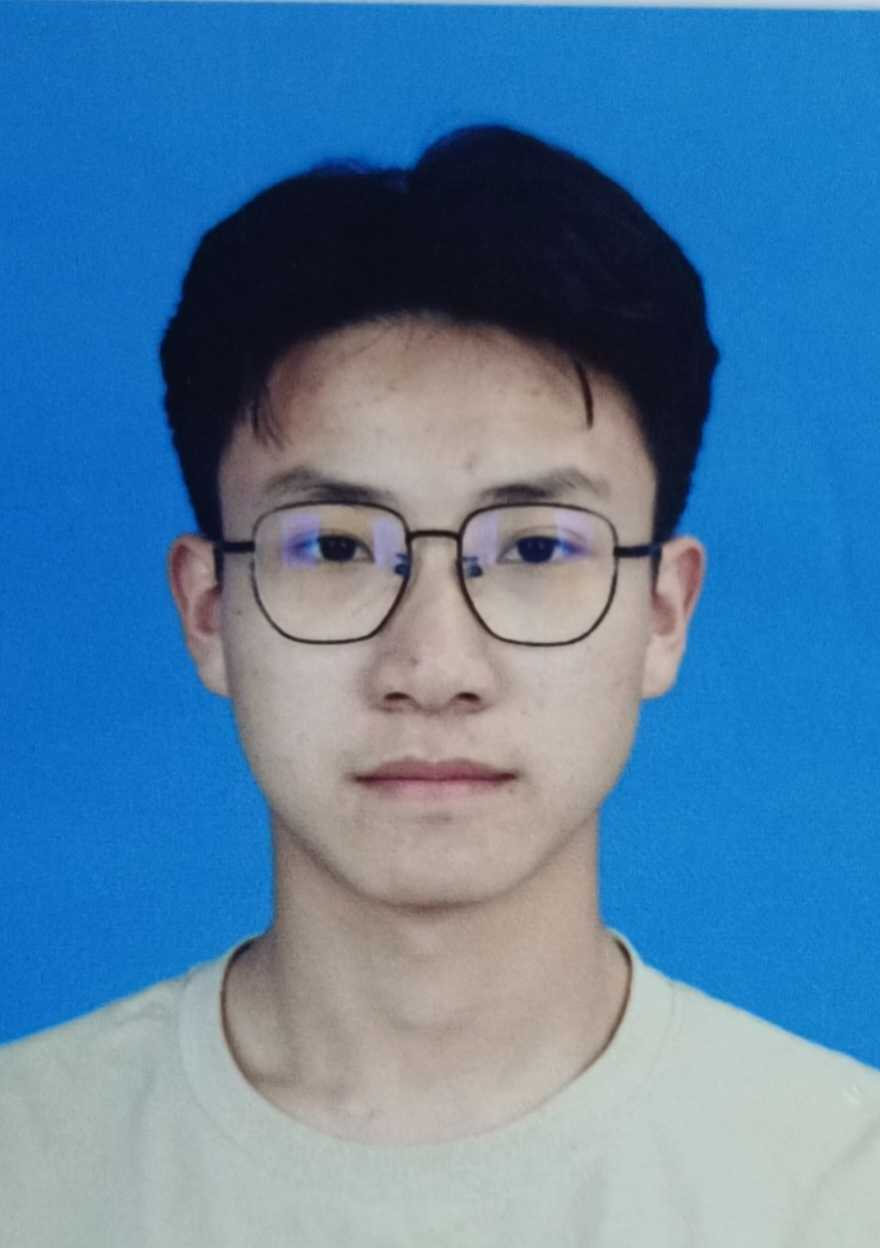
\includegraphics[height=2.2cm]{assets/portrait-user.jpg}
\end{minipage}
\vspace{2pt}

% ==================== Education ====================
\section*{\educationicon\hspace{0.38em}Education}
\noindent
\textbf{University of Electronic Science and Technology of China (UESTC)} \hfill \textbf{2024.9 - 2028.6} \\
\textbf{Yingcai Honors College} \quad \textbf{Major: }Fundamental Science of Mathematics \& Physics (Elite Talent Class) \quad \textbf{Focus: }AI \\
\textbf{GPA: 3.96/4.0 \quad Weighted Average: 91.55 \quad Rank: 2/24 \quad CET-4: 581 \quad CET-6: 561} \\
\textbf{Core Courses: }Advanced Calculus, Advanced Algebra and Geometry, University Physics, Probability and Mathematical Statistics, Data Structures, Advanced Programming Language Design, Machine Learning, etc.

% ==================== Research Experience ====================
\section*{\researchicon\hspace{0.38em}Research Experience}

\researchentry{Computational Pathology \& Multiple Instance Learning}{2025.3 - 2025.8}{CKMIL: Cascaded Key-Instance Attention Multiple Instance Learning for Histopathology Whole Slide Image Analysis {\normalfont\href{https://haoceanlab.cn/pdfs/ckmil-aaai-26.pdf}{[pdf]}}{\normalfont\color{black}\hfill\mbox{Submitted to AAAI 2026\quad\textbf{First Author}}}}
\textbf{Advisors: }Prof. Liang-Jian Deng, School of Mathematical Sciences, UESTC \qquad Asst. Prof. Hao Chen, HKUST
\begin{itemize}[leftmargin=*, nosep, itemsep=2pt]
    \item Proposed CKMIL, a cascaded key-instance attention framework for whole slide images (WSIs) with sparse diagnostic signals, using key instances to guide efficient dependency modeling; achieved leading results on multi-cohort cancer subtyping and survival prediction (BRACS, TCGA).
    \item \textbf{Contribution: }Project lead; drove data processing, method design, experiments, and paper writing.
\end{itemize}
\projectseparator
\projectheading{LVLM Safety \& Jailbreak Attacks}{2025.9 - 2025.12}
\paperentry{Persuasion in Scene: A Multi-Agent Typographic Jailbreak Crew against Large Vision-Language Models}{{\normalfont\href{https://haoceanlab.cn/pdfs/persuasion-in-scene-cvpr-2026.pdf}{[pdf]}}}{Submitted to CVPR 2026}{Co-First Author}
\paperentry{Models as Lego Builders: Assembling Malice from Benign Blocks via Semantic Blueprints}{{\normalfont\href{https://arxiv.org/pdf/2603.07590}{[pdf]}}}{Accepted by CVPR 2026}{Third Author}
\begin{itemize}[leftmargin=*, nosep, itemsep=2pt]
    \item Proposed PIS, a multi-agent cross-modal jailbreak framework, and StructAttack, a single-shot, optimization-free attack via semantic slot-filling, both achieving leading attack success rates on open- and closed-source LVLMs.
    \item \textbf{Contribution: }As co-first author of PIS, contributed centrally to ideation, method design, experiments, and writing; as third author of StructAttack, adapted and evaluated the method on SafeBench.
\end{itemize}
\projectseparator
\projectheading{Pathology Foundation Models \& Efficient WSI Analysis}{2025.12 - Present}
\paperentry{From Full-Bag Diagnosis to Budgeted Patch Selection: Role-Decoupled Benchmarking and Adaptation of}{Pathology Foundation Models in Whole-Slide Imaging}{Target: IEEE TMI 2027}{First Author}
\noindent\textbf{Advisors: }Prof. Liang-Jian Deng, School of Mathematical Sciences, UESTC \qquad Asst. Prof. Hao Chen, HKUST
\begin{itemize}[leftmargin=*, nosep, itemsep=2pt]
    \item Found that some morphological tasks need no image reconstruction, due to image redundancy and foundation model (FM) robustness; studied FM capability decoupling in Selector$\times$Consumer settings and proposed adaptation fixes.
\end{itemize}
\projectseparator
\projectheading{Multimodal Post-Training \& CoT Reasoning}{2026.4 - 2026.10}
\paperentry{ReMAP: Restoring the Perceptual Cycle with Reasoning-Time Latent Visual Memory}{{\normalfont\color{black}\textbf{Advisor: }Shanghang Zhang, Peking University}}{Submitted to ICLR 2027}{First Author}
\begin{itemize}[leftmargin=*, nosep, itemsep=2pt]
    \item Analyzed reasoning-time visual memory along curation, organization, and access: local evidence needs global context, compact latents balance accuracy and cost, and access utility depends on the reasoning state.
    \item Proposed ReMAP, coupling a question-conditioned Global memory with a state-guided Local memory returned as compact latent tokens, plus an RL access policy trained via branched rollouts; leads across ten benchmark families, beats the prior best on MuirBench/MIMIC by 8.38/14.84 points, and cuts visual tokens by 51.0--76.8\%.
\end{itemize}

% ==================== Skills ====================
\section*{\skillsicon\hspace{0.38em}Skills}
\begin{itemize}[leftmargin=*, nosep, itemsep=2pt]
    \item \textbf{Tools: }Python, PyTorch, Linux, Git, LaTeX, Codex, Claude Code; idea validation, experiments, writing.
    \item \textbf{Deep Learning: }Transformer, Mamba; test-time training, post-training, and evaluation of multimodal LLMs.
\end{itemize}

% ==================== Honors & Awards ====================
\section*{\awardicon\hspace{0.38em}Honors \& Awards}
\begin{itemize}[leftmargin=*, nosep, itemsep=2pt]
    \item UESTC Outstanding Student Scholarship \quad First Class \hfill \textbf{2025}
    \item UESTC Outstanding Student Scholarship \quad First Class \hfill \textbf{2026}
    \item Mathematical Contest in Modeling (MCM/ICM) \quad Meritorious Winner \hfill \textbf{2026}
    \item UESTC (iFLYTEK Cup) 1st AI Agent Creativity Competition \quad First Prize \hfill \textbf{2026}
\end{itemize}

\end{document}
